\documentclass{article}
% if you need to pass options to natbib, use, e.g.:
%     \PassOptionsToPackage{numbers, compress}{natbib}
% before loading neurips_2023
\usepackage[final]{neurips}
% to avoid loading the natbib package, add option nonatbib:
%    \usepackage[nonatbib]{neurips}


\usepackage[utf8]{inputenc} % allow utf-8 input
\usepackage[T1]{fontenc}    % use 8-bit T1 fonts
\usepackage{hyperref}       % hyperlinks
\usepackage{url}            % simple URL typesetting
\usepackage{booktabs}       % professional-quality tables
\usepackage{amsfonts}       % blackboard math symbols
\usepackage{nicefrac}       % compact symbols for 1/2, etc.
\usepackage{microtype}      % microtypography
\usepackage{xcolor}         % colors
\usepackage{graphicx}       % include graphics
\usepackage{subcaption}     % subfigures
\usepackage{amsmath}        % math environments
\usepackage{algorithm}      % algorithm environment
\usepackage{algorithmic}    % algorithmic pseudo-code


\title{Predicting Canadian Dollar Exchange Rates Against Major Global Currencies Using Machine Learning}


\author{%
  Member 1\\
  Department of Electrical \& Computer Engineering\\
  University of Toronto\\
  \texttt{member1@mail.utoronto.ca} \\
  \And
  Member 2\\
  Department of Electrical \& Computer Engineering\\
  University of Toronto\\
  \texttt{member2@mail.utoronto.ca} \\
  \And
  Member 3\\
  Department of Electrical \& Computer Engineering\\
  University of Toronto\\
  \texttt{member3@mail.utoronto.ca} \\
}

\begin{document}


\maketitle


\begin{abstract}
We study next-day prediction of the Canadian dollar (CAD) exchange rate against three major currencies---USD, EUR, and CNY---using daily data from the Bank of Canada. The task is formulated as supervised regression with 23 engineered features (lagged values, rolling statistics, returns, and cyclical date encodings). We compare ordinary least-squares linear regression, support vector regression (SVR) with an RBF kernel, and a multilayer perceptron (MLP) in PyTorch. Linear regression achieves the best performance across all pairs ($R^2 > 0.94$), while SVR and MLP underperform due to a feature--target scale mismatch. We analyze these results and propose improvements including target normalization and recurrent architectures.
\end{abstract}

\section*{Attestation of Teamwork}
All three team members contributed equally to all stages of this project, including problem formulation, model design and implementation, experimentation, and report writing.


\section{Introduction}

Exchange-rate forecasting is a central problem in computational finance, supporting hedging, trade pricing, and policy analysis~[1]. The Canadian dollar is of particular interest because Canada is a major trading partner of the United States, the European Union, and China. Traditional econometric approaches such as the random-walk model remain difficult-to-beat baselines~[2], but advances in machine learning have renewed interest in data-driven forecasting, with nonlinear models showing promise on financial time series~[3,~4].

We investigate whether supervised learning methods can identify predictive structure in daily CAD exchange-rate data against three currencies (USD, EUR, CNY), comparing linear regression with SVR and an MLP.


\section{Preliminaries and Problem Formulation}

\subsection{Problem Setting}

We consider the task of predicting the next-day exchange rate of the Canadian dollar against a target currency. Let $r_t$ denote the exchange rate on business day $t$. Given a feature vector $\mathbf{x}_t \in \mathbb{R}^d$ constructed from historical observations up to and including day $t$, we seek a function $f: \mathbb{R}^d \rightarrow \mathbb{R}$ such that:
\begin{equation}
  \hat{r}_{t+1} = f(\mathbf{x}_t)
\end{equation}
where $\hat{r}_{t+1}$ is the predicted exchange rate for day $t+1$.

\subsection{Feature Construction}

The feature vector $\mathbf{x}_t$ consists of 23 engineered features derived from the raw exchange-rate time series:

\begin{itemize}
  \item \textbf{Lag features}: $r_{t-k}$ for $k \in \{1, 2, 3, 5, 7, 10, 14, 21\}$, providing the model with recent price history at multiple time scales.
  \item \textbf{Rolling statistics}: The rolling mean $\bar{r}_{t}^{(w)}$ and rolling standard deviation $\sigma_{t}^{(w)}$ computed over windows $w \in \{5, 10, 21, 50\}$ business days (shifted by one day to avoid look-ahead bias).
  \item \textbf{Percentage changes}: The 1-day and 5-day returns, $\Delta r_t^{(1)} = (r_t - r_{t-1})/r_{t-1}$ and $\Delta r_t^{(5)} = (r_t - r_{t-5})/r_{t-5}$.
  \item \textbf{Cyclical date encodings}: Sine and cosine transformations of the day-of-week ($\sin(2\pi d/5)$, $\cos(2\pi d/5)$) and month ($\sin(2\pi m/12)$, $\cos(2\pi m/12)$) to capture calendar seasonality without introducing ordinal artifacts.
\end{itemize}

\subsection{Evaluation Metrics}

We evaluate model performance using three standard regression metrics:
\begin{align}
  \text{MAE} &= \frac{1}{n}\sum_{i=1}^{n} |r_i - \hat{r}_i| \\
  \text{RMSE} &= \sqrt{\frac{1}{n}\sum_{i=1}^{n} (r_i - \hat{r}_i)^2} \\
  R^2 &= 1 - \frac{\sum_{i=1}^{n}(r_i - \hat{r}_i)^2}{\sum_{i=1}^{n}(r_i - \bar{r})^2}
\end{align}
where $r_i$ and $\hat{r}_i$ are the actual and predicted values, $\bar{r}$ is the mean of the actual values, and $n$ is the number of test samples.

	
\section{Design}

Our system follows a modular pipeline design consisting of five stages, as illustrated in Figure~\ref{fig:pipeline}.

\begin{figure}[!t]
  \centering
  \fbox{%
    \parbox{0.9\textwidth}{\centering
      \textbf{Data Download} $\rightarrow$ \textbf{Feature Engineering} $\rightarrow$ \textbf{Train/Val/Test Split} $\rightarrow$ \textbf{Model Training} $\rightarrow$ \textbf{Evaluation \& Visualization}
    }%
  }
  \caption{High-level pipeline architecture.}
  \label{fig:pipeline}
\end{figure}

The pipeline comprises five modules: (1)~\textbf{Data Loader} downloads daily data from the Bank of Canada Valet API for USD/CAD, EUR/CAD, and CNY/CAD (2015--2025; 2,244 observations each); (2)~\textbf{Preprocessing} constructs 23 features (Section~2.2), performs a chronological 70/15/15 split, and applies standard scaling fitted on the training set only; (3)~\textbf{Models} implements Linear Regression, SVR (scikit-learn), and MLP (PyTorch); (4)~\textbf{Training} handles fitting with early stopping for the MLP; (5)~\textbf{Evaluation} computes metrics and generates figures.


\section{Methodology}

\subsection{Linear Regression (Baseline)}

Ordinary least-squares (OLS) linear regression serves as our baseline. The model assumes a linear relationship between features and the target:
\begin{equation}
  \hat{r}_{t+1} = \mathbf{w}^\top \mathbf{x}_t + b
\end{equation}
where $\mathbf{w} \in \mathbb{R}^d$ and $b \in \mathbb{R}$ are learned by minimizing the sum of squared residuals. We use the \texttt{LinearRegression} class from scikit-learn~[5].

\subsection{Support Vector Regression (SVR)}

SVR finds a function that deviates from the training targets by at most $\varepsilon$ while remaining as flat as possible~[6]. We use the radial basis function (RBF) kernel:
\begin{equation}
  K(\mathbf{x}_i, \mathbf{x}_j) = \exp\!\left(-\gamma \|\mathbf{x}_i - \mathbf{x}_j\|^2\right)
\end{equation}
with hyperparameters $C = 10$, $\varepsilon = 0.01$, and $\gamma = \text{scale}$ (i.e., $\gamma = 1/(d \cdot \text{Var}(\mathbf{X}))$). The implementation uses the \texttt{SVR} class from scikit-learn.

\subsection{Multilayer Perceptron (MLP)}

The MLP is a feedforward neural network implemented in PyTorch~[7]. The architecture consists of three hidden layers with 128, 64, and 32 neurons respectively. Each hidden layer applies the following sequence of operations:

\begin{equation}
  \mathbf{h}^{(l)} = \text{Dropout}\!\Big(\text{ReLU}\!\big(\text{BatchNorm}(\mathbf{W}^{(l)} \mathbf{h}^{(l-1)} + \mathbf{b}^{(l)})\big)\Big)
\end{equation}

The output layer is a single linear neuron producing the scalar prediction $\hat{r}_{t+1}$.

\begin{algorithm}[!t]
\caption{MLP Training with Early Stopping}
\label{alg:mlp}
\begin{algorithmic}[1]
\REQUIRE Training data $(\mathbf{X}_{\text{train}}, \mathbf{y}_{\text{train}})$, validation data $(\mathbf{X}_{\text{val}}, \mathbf{y}_{\text{val}})$, patience $P$
\STATE Initialize MLP parameters $\theta$
\STATE $\text{best\_loss} \leftarrow \infty$, $\text{counter} \leftarrow 0$
\FOR{epoch $= 1, 2, \ldots, E_{\max}$}
  \FOR{each mini-batch $(\mathbf{X}_b, \mathbf{y}_b)$ from training set}
    \STATE $\hat{\mathbf{y}}_b \leftarrow \text{MLP}_\theta(\mathbf{X}_b)$
    \STATE $\mathcal{L} \leftarrow \text{MSE}(\hat{\mathbf{y}}_b, \mathbf{y}_b)$
    \STATE $\theta \leftarrow \theta - \eta \nabla_\theta \mathcal{L}$ \COMMENT{Adam optimizer}
  \ENDFOR
  \STATE Compute $\mathcal{L}_{\text{val}}$ on validation set
  \IF{$\mathcal{L}_{\text{val}} < \text{best\_loss}$}
    \STATE $\text{best\_loss} \leftarrow \mathcal{L}_{\text{val}}$, save $\theta^*$, $\text{counter} \leftarrow 0$
  \ELSE
    \STATE $\text{counter} \leftarrow \text{counter} + 1$
  \ENDIF
  \IF{$\text{counter} \geq P$}
    \STATE \textbf{break} \COMMENT{Early stopping}
  \ENDIF
\ENDFOR
\RETURN $\theta^*$
\end{algorithmic}
\end{algorithm}

\textbf{Training details:} The MLP is trained using the Adam optimizer~[8] with learning rate $\eta = 10^{-3}$, weight decay $10^{-5}$, batch size 64, and a maximum of 200 epochs. A \texttt{ReduceLROnPlateau} scheduler halves the learning rate if validation loss does not improve for 10 epochs. Early stopping with patience $P = 20$ epochs prevents overfitting. Dropout rate is set to 0.2.

\textbf{Libraries:} We use Python 3.14, PyTorch 2.0+ for the MLP, scikit-learn 1.3+ for Linear Regression and SVR, pandas for data manipulation, and matplotlib for visualization.


\section{Numerical Experiments}

\subsection{Dataset and Experimental Setup}

We use daily exchange-rate data from the Bank of Canada Valet API (January 2015--December 2025), yielding 2,244 observations per pair. After a 50-day warm-up for rolling features, 2,193 samples remain. These are split chronologically: 1,535 training (70\%), 329 validation (15\%), 329 test (15\%), covering approximately August 2024 to January 2026. All features are standardized using a \texttt{StandardScaler} fitted on the training set only. Seeds are fixed to 42 for reproducibility.

\subsection{Results}

Table~\ref{tab:results} summarizes the performance of all three models on the test set across the three currency pairs.

\begin{table}[!t]
  \caption{Test-set performance across all currency pairs and models.}
  \label{tab:results}
  \centering
  \begin{tabular}{llccc}
    \toprule
    Currency & Model & MAE & RMSE & $R^2$ \\
    \midrule
    USD/CAD & Linear Regression & 0.0033 & 0.0045 & 0.9707 \\
    USD/CAD & SVR               & 0.0294 & 0.0369 & $-$0.9733 \\
    USD/CAD & MLP               & 0.0539 & 0.0636 & $-$4.8678 \\
    \midrule
    EUR/CAD & Linear Regression & 0.0041 & 0.0053 & 0.9907 \\
    EUR/CAD & SVR               & 0.0243 & 0.0360 & 0.5684 \\
    EUR/CAD & MLP               & 0.0660 & 0.0797 & $-$1.1139 \\
    \midrule
    CNY/CAD & Linear Regression & 0.0004 & 0.0006 & 0.9496 \\
    CNY/CAD & SVR               & 0.0023 & 0.0028 & $-$0.0455 \\
    CNY/CAD & MLP               & 0.0021 & 0.0025 & 0.1753 \\
    \bottomrule
  \end{tabular}
\end{table}

\subsection{Prediction Plots}

Figure~\ref{fig:predictions} shows actual vs.\ predicted exchange rates on the test set for all three currency pairs.

\begin{figure}[!t]
  \centering
  \begin{subfigure}[b]{\textwidth}
    \centering
    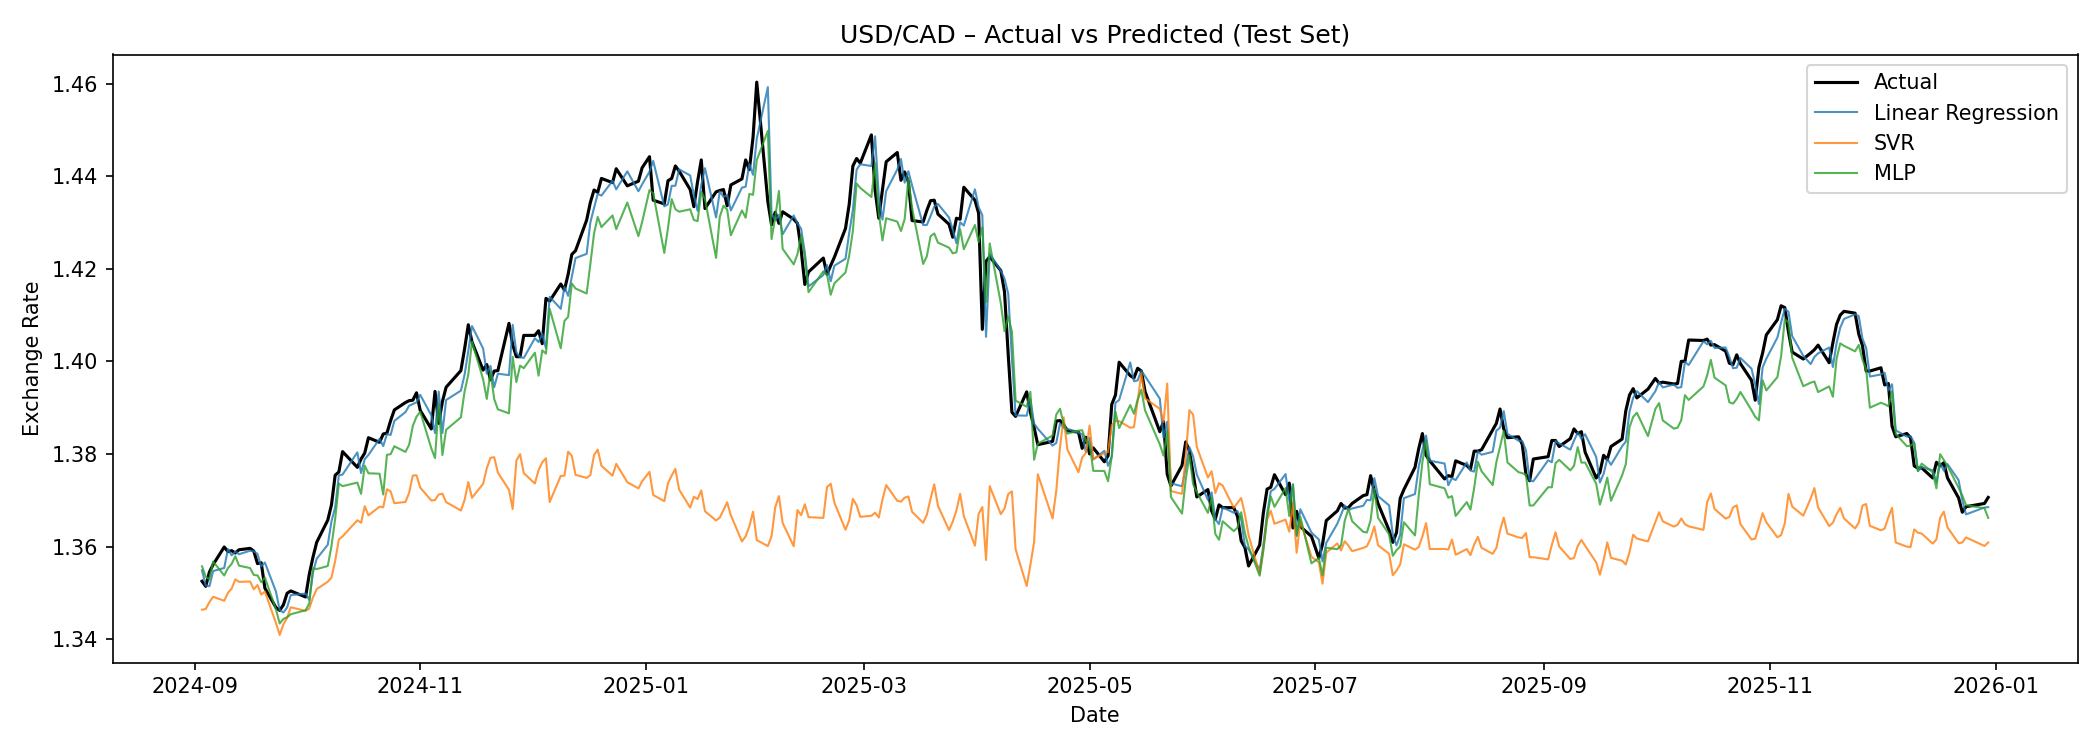
\includegraphics[width=\textwidth]{figures/USD_predictions.png}
    \caption{USD/CAD}
    \label{fig:usd_pred}
  \end{subfigure}\\[4pt]
  \begin{subfigure}[b]{\textwidth}
    \centering
    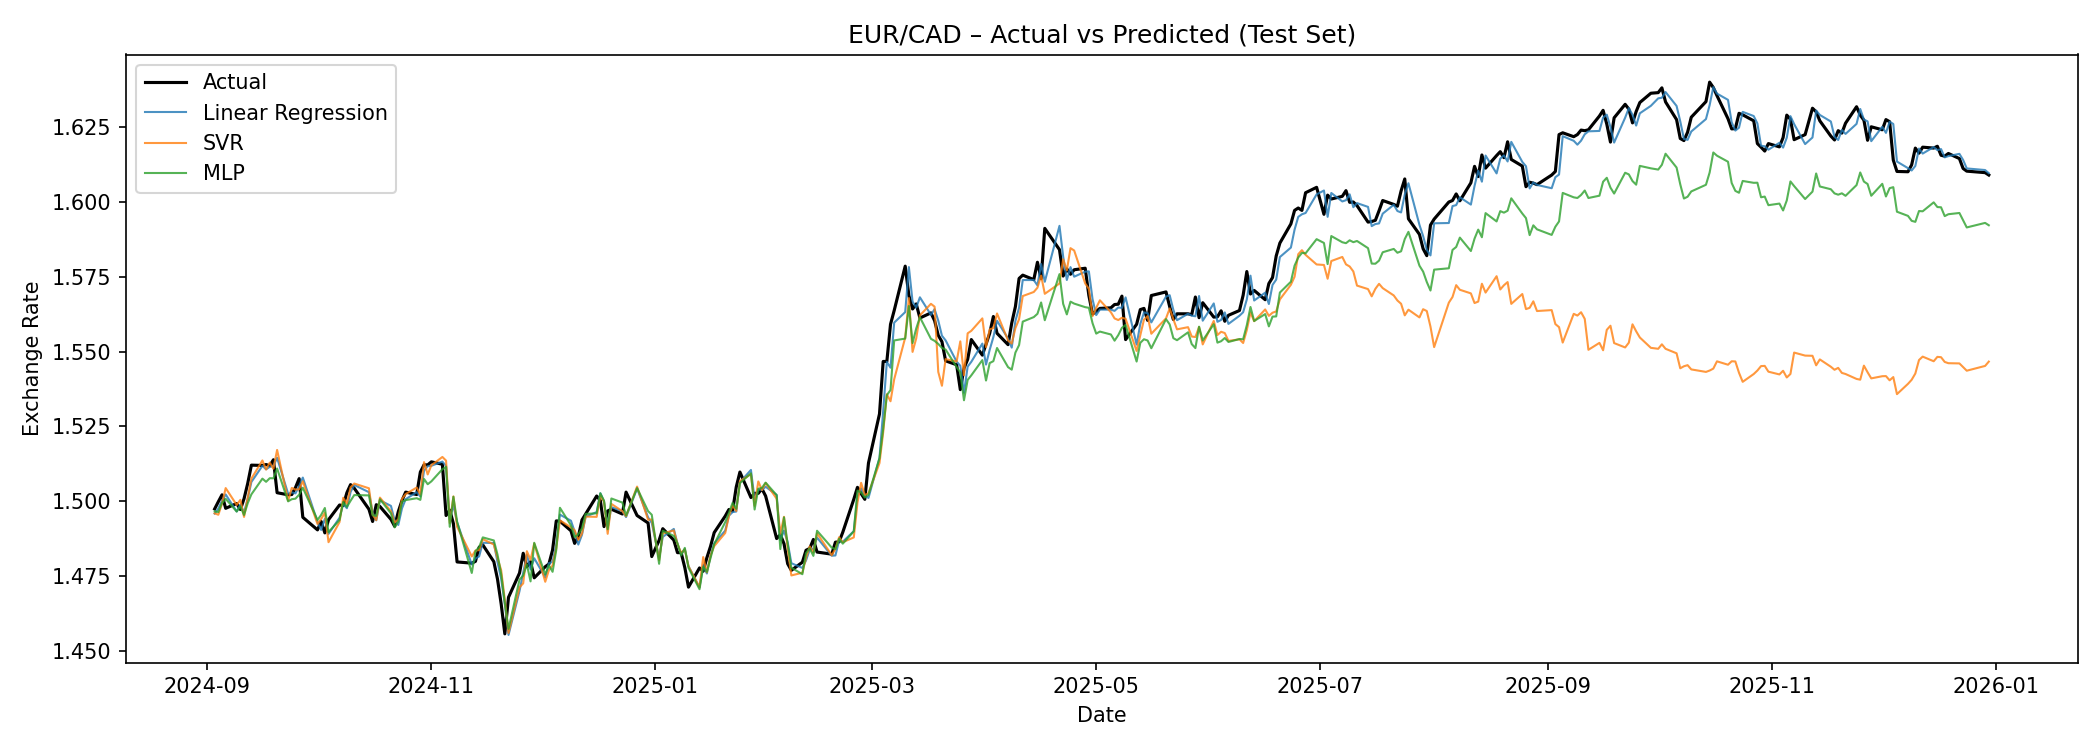
\includegraphics[width=\textwidth]{figures/EUR_predictions.png}
    \caption{EUR/CAD}
    \label{fig:eur_pred}
  \end{subfigure}\\[4pt]
  \begin{subfigure}[b]{\textwidth}
    \centering
    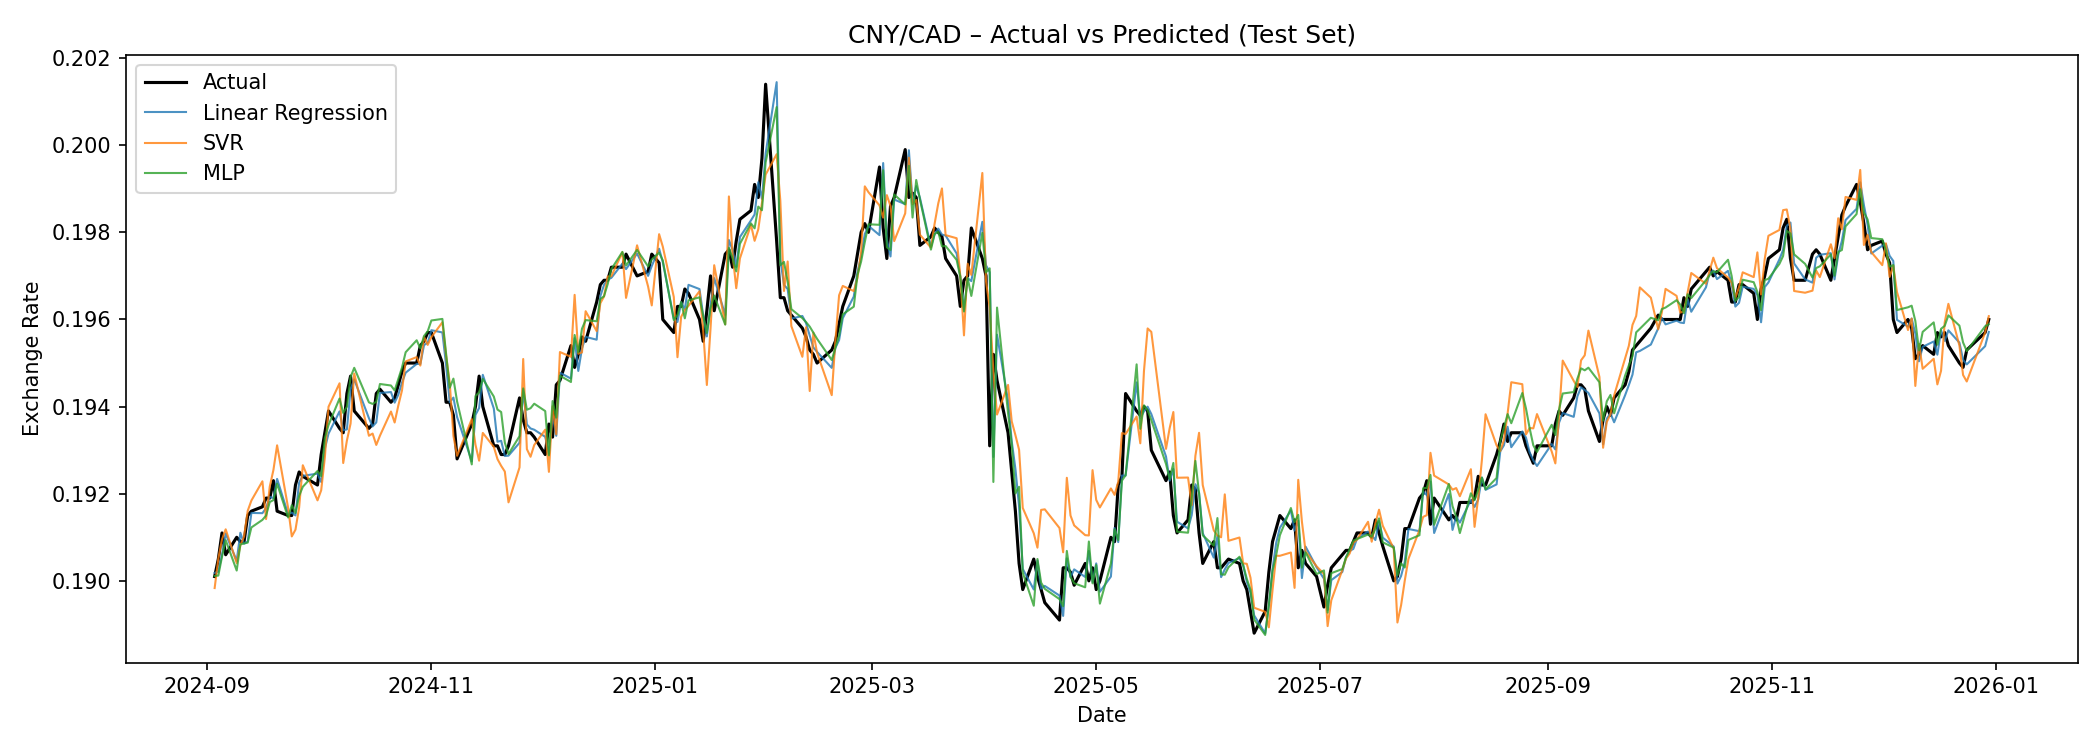
\includegraphics[width=\textwidth]{figures/CNY_predictions.png}
    \caption{CNY/CAD}
    \label{fig:cny_pred}
  \end{subfigure}
  \caption{Actual vs.\ predicted exchange rates on the test set. Linear Regression (blue) tracks actual values (black) closely. SVR (orange) tends toward near-constant predictions, and MLP (green) exhibits high variance.}
  \label{fig:predictions}
\end{figure}

\subsection{Learning Curves}

Figure~\ref{fig:learning_curves} shows the MLP training and validation loss curves.

\begin{figure}[!t]
  \centering
  \begin{subfigure}[b]{0.32\textwidth}
    \centering
    
\includegraphics[width=\textwidth]{figures/USD_learning_curve.png}
    \caption{USD/CAD}
    \label{fig:usd_lc}
  \end{subfigure}\hfill
  \begin{subfigure}[b]{0.32\textwidth}
    \centering
    
\includegraphics[width=\textwidth]{figures/EUR_learning_curve.png}
    \caption{EUR/CAD}
    \label{fig:eur_lc}
  \end{subfigure}\hfill
  \begin{subfigure}[b]{0.32\textwidth}
    \centering
    
\includegraphics[width=\textwidth]{figures/CNY_learning_curve.png}
    \caption{CNY/CAD}
    \label{fig:cny_lc}
  \end{subfigure}
  \caption{MLP learning curves. Train and validation loss converge quickly in all cases; a persistent gap indicates some overfitting. Early stopping triggered at epochs 84 (USD), 101 (EUR), and 79 (CNY).}
  \label{fig:learning_curves}
\end{figure}

Key hyperparameters: SVR uses an RBF kernel with $C=10$, $\varepsilon=0.01$, $\gamma=\text{scale}$. The MLP has hidden layers $[128, 64, 32]$ with ReLU, batch normalization, and dropout (0.2), trained with Adam ($\eta=10^{-3}$, weight decay $10^{-5}$), batch size 64, and early stopping (patience 20). Full details are in Table~\ref{tab:hyperparams} (Appendix).


\section{Discussion}

\subsection{Linear Regression Dominates}

Linear regression achieved $R^2$ values of 0.97 (USD), 0.99 (EUR), and 0.95 (CNY). The most predictive feature is the 1-day lag ($r_{t-1}$); the linear model effectively approximates a random-walk-plus-drift model, a well-known strong baseline~[2].

\subsection{SVR and MLP Underperformance}

Both SVR and MLP underperformed due to a \textbf{feature--target scale mismatch}: input features were standardized but the target was left in its original scale. For SVR, the $\varepsilon$-insensitive tube ($\varepsilon=0.01$) encompasses most natural variation in USD/CAD ($\approx 1.4$), producing near-constant predictions. For the MLP, outputting raw exchange rates from standardized inputs creates unstable gradients.

The CNY/CAD pair ($\approx 0.19$) yielded the best MLP results ($R^2 = 0.175$), consistent with a less severe scale mismatch. EUR/CAD benefited SVR ($R^2 = 0.57$) due to its larger signal amplitude relative to $\varepsilon$.

\subsection{Summary}

Lag features contain strong predictive signal for next-day rates, but this is largely autoregressive rather than revealing complex nonlinear structure. With proper target normalization, nonlinear models may match or modestly improve upon the linear baseline.


\section{Conclusions}

Linear regression achieves $R^2 > 0.94$ on all three currency pairs by leveraging strong autocorrelation in exchange-rate series. SVR and MLP underperformed due to a feature--target scale mismatch, underscoring the importance of consistent preprocessing. The dominant predictive signal comes from the most recent lag values.

\textbf{Future work:} (a)~Normalizing the target alongside features, (b)~systematic hyperparameter tuning, (c)~recurrent or Transformer architectures, (d)~exogenous features (interest rates, commodities), and (e)~direction-of-change classification.


\section*{References}

\medskip
{
\small

[1] Meese, R.A.\ \& Rogoff, K.\ (1983) Empirical exchange rate models of the seventies: Do they fit out of sample? {\it Journal of International Economics} {\bf 14}(1--2):3--24.

[2] Rossi, B.\ (2013) Exchange rate predictability. {\it Journal of Economic Literature} {\bf 51}(4):1063--1119.

[3] Vapnik, V.N.\ (1995) {\it The Nature of Statistical Learning Theory.} New York: Springer-Verlag.

[4] Hornik, K., Stinchcombe, M.\ \& White, H.\ (1989) Multilayer feedforward networks are universal approximators. {\it Neural Networks} {\bf 2}(5):359--366.

[5] Pedregosa, F.\ et al.\ (2011) Scikit-learn: Machine learning in Python. {\it Journal of Machine Learning Research} {\bf 12}:2825--2830.

[6] Smola, A.J.\ \& Sch\"olkopf, B.\ (2004) A tutorial on support vector regression. {\it Statistics and Computing} {\bf 14}(3):199--222.

[7] Paszke, A.\ et al.\ (2019) PyTorch: An imperative style, high-performance deep learning library. In {\it Advances in Neural Information Processing Systems 32}, pp.\ 8026--8037.

[8] Kingma, D.P.\ \& Ba, J.\ (2015) Adam: A method for stochastic optimization. In {\it Proc.\ 3rd International Conference on Learning Representations (ICLR)}.

[9] Bank of Canada (2025) Valet API documentation. \url{https://www.bankofcanada.ca/valet/docs}.
}

\section*{Appendix}

\subsection*{A. Hyperparameters}

\begin{table}[h]
  \caption{Hyperparameters for SVR and MLP models.}
  \label{tab:hyperparams}
  \centering
  \begin{tabular}{lll}
    \toprule
    Model & Parameter & Value \\
    \midrule
    SVR & Kernel & RBF \\
    SVR & $C$ & 10.0 \\
    SVR & $\varepsilon$ & 0.01 \\
    SVR & $\gamma$ & scale \\
    \midrule
    MLP & Hidden layers & [128, 64, 32] \\
    MLP & Activation & ReLU \\
    MLP & Dropout rate & 0.2 \\
    MLP & Batch normalization & Yes \\
    MLP & Optimizer & Adam \\
    MLP & Learning rate & $10^{-3}$ \\
    MLP & Weight decay & $10^{-5}$ \\
    MLP & Batch size & 64 \\
    MLP & Max epochs & 200 \\
    MLP & Early stopping patience & 20 \\
    MLP & LR scheduler & ReduceLROnPlateau (factor=0.5, patience=10) \\
    \bottomrule
  \end{tabular}
\end{table}

\subsection*{B. Residual Histograms}

Figure~\ref{fig:residuals} shows residual distributions for all model--currency combinations. Linear Regression residuals are tightly centered around zero, while SVR and MLP exhibit wider, often biased residual distributions.

\begin{figure}[h]
  \centering
  \begin{subfigure}[b]{0.32\textwidth}
    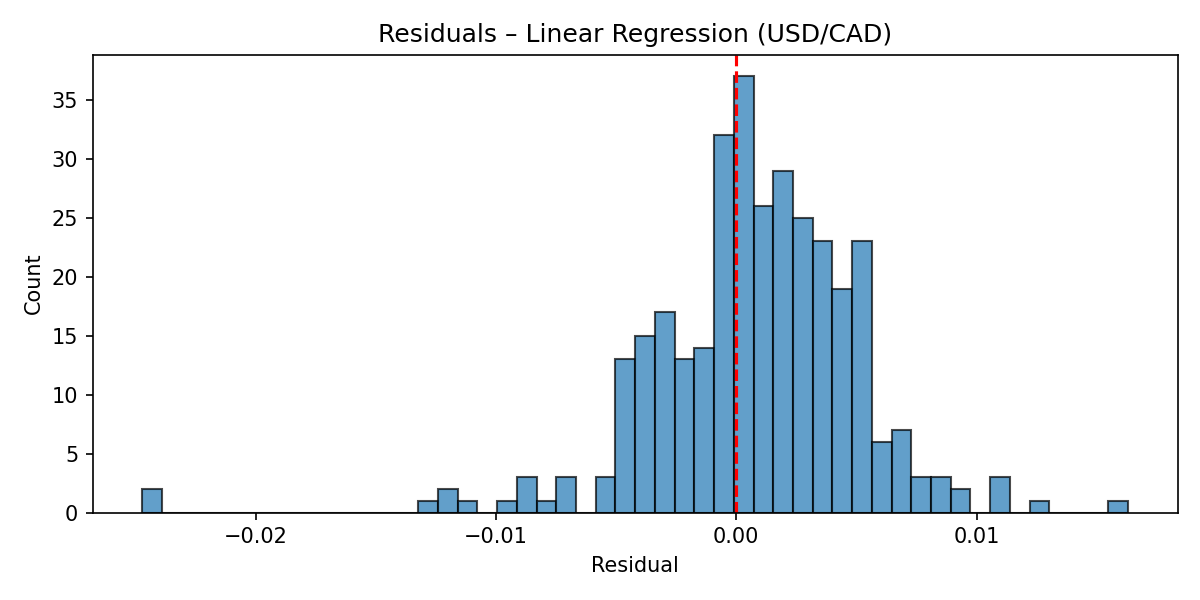
\includegraphics[width=\textwidth]{figures/USD_Linear_Regression_residuals.png}
    \caption{LR -- USD}
  \end{subfigure}\hfill
  \begin{subfigure}[b]{0.32\textwidth}
    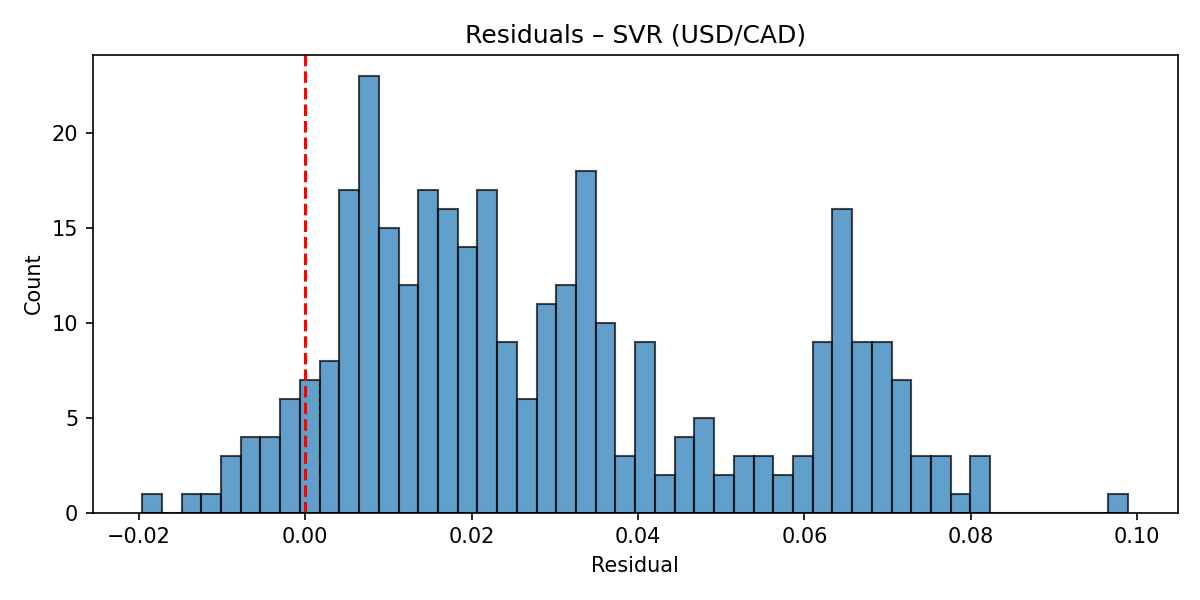
\includegraphics[width=\textwidth]{figures/USD_SVR_residuals.png}
    \caption{SVR -- USD}
  \end{subfigure}\hfill
  \begin{subfigure}[b]{0.32\textwidth}
    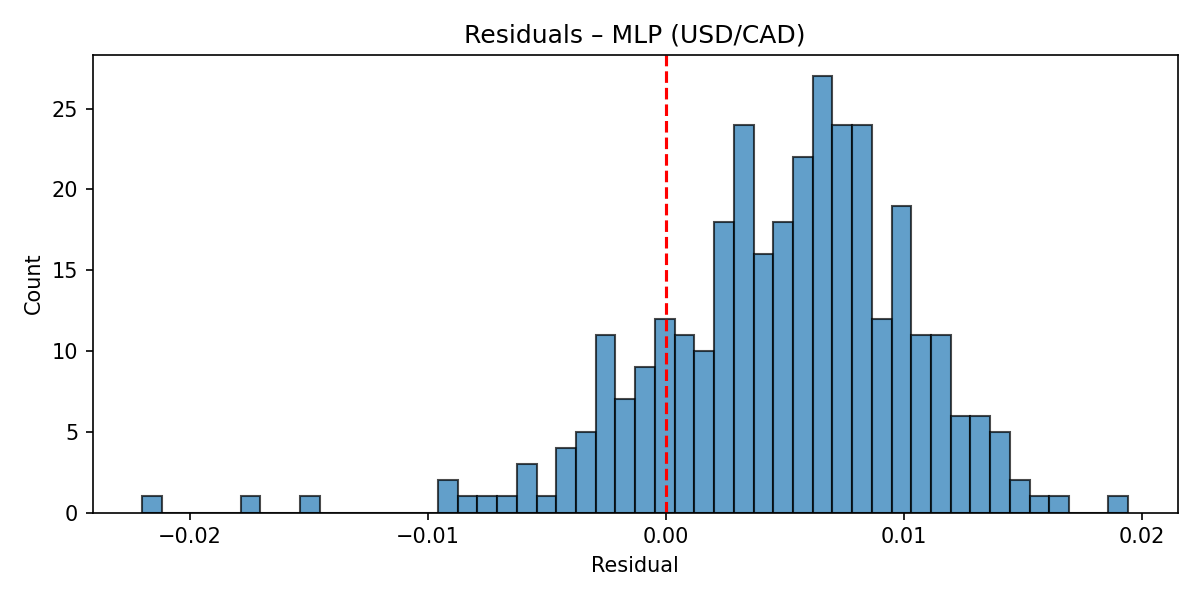
\includegraphics[width=\textwidth]{figures/USD_MLP_residuals.png}
    \caption{MLP -- USD}
  \end{subfigure}\\[4pt]
  \begin{subfigure}[b]{0.32\textwidth}
    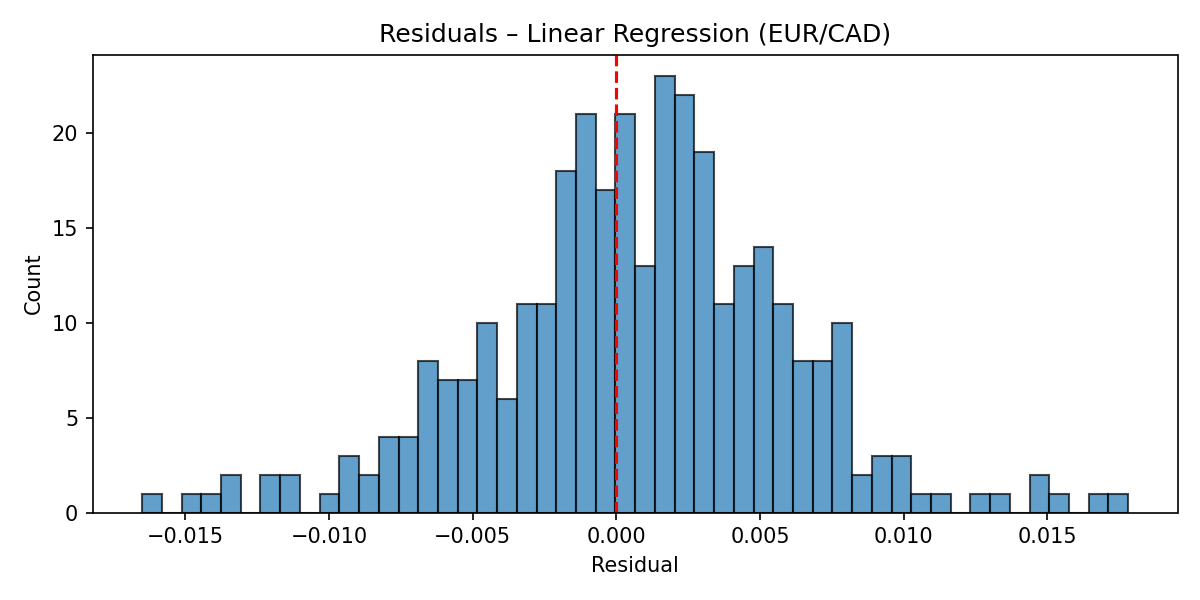
\includegraphics[width=\textwidth]{figures/EUR_Linear_Regression_residuals.png}
    \caption{LR -- EUR}
  \end{subfigure}\hfill
  \begin{subfigure}[b]{0.32\textwidth}
    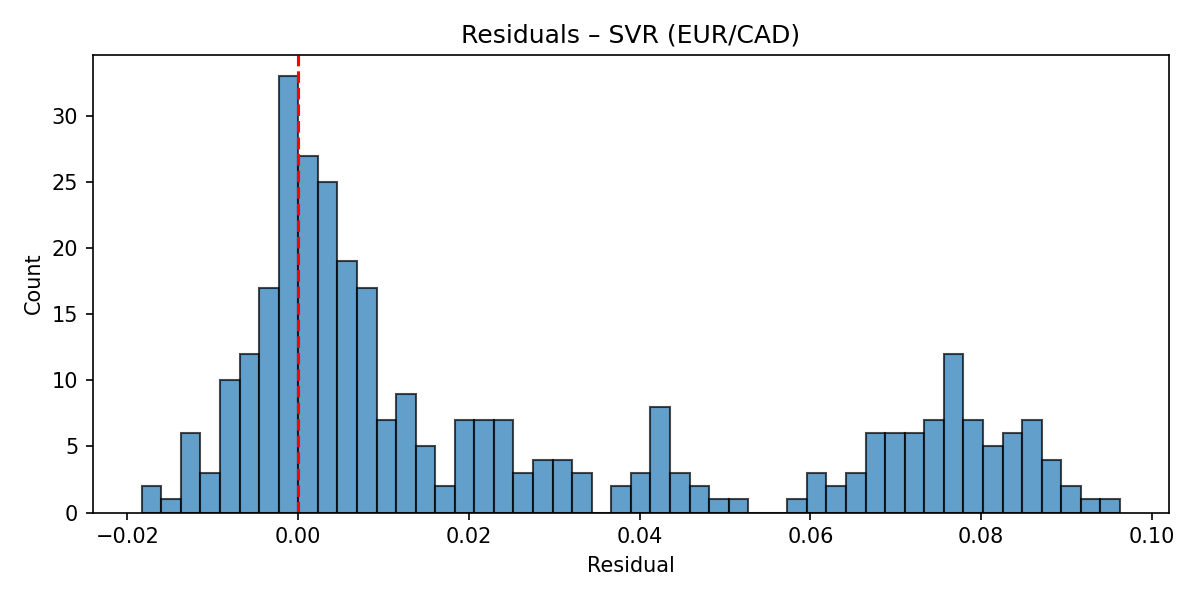
\includegraphics[width=\textwidth]{figures/EUR_SVR_residuals.png}
    \caption{SVR -- EUR}
  \end{subfigure}\hfill
  \begin{subfigure}[b]{0.32\textwidth}
    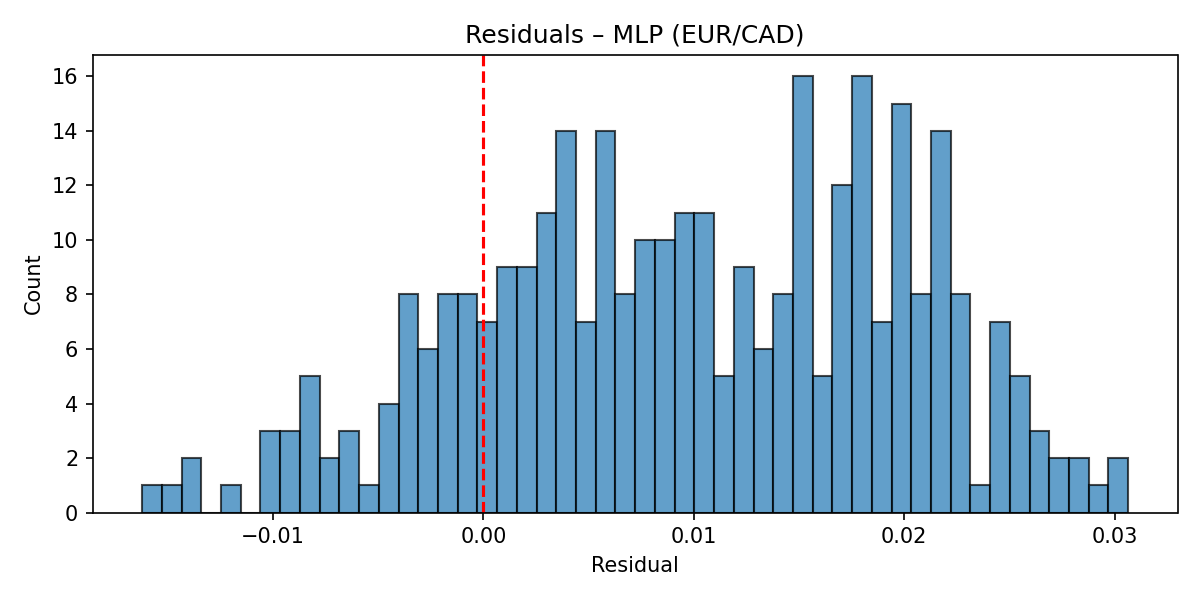
\includegraphics[width=\textwidth]{figures/EUR_MLP_residuals.png}
    \caption{MLP -- EUR}
  \end{subfigure}\\[4pt]
  \begin{subfigure}[b]{0.32\textwidth}
    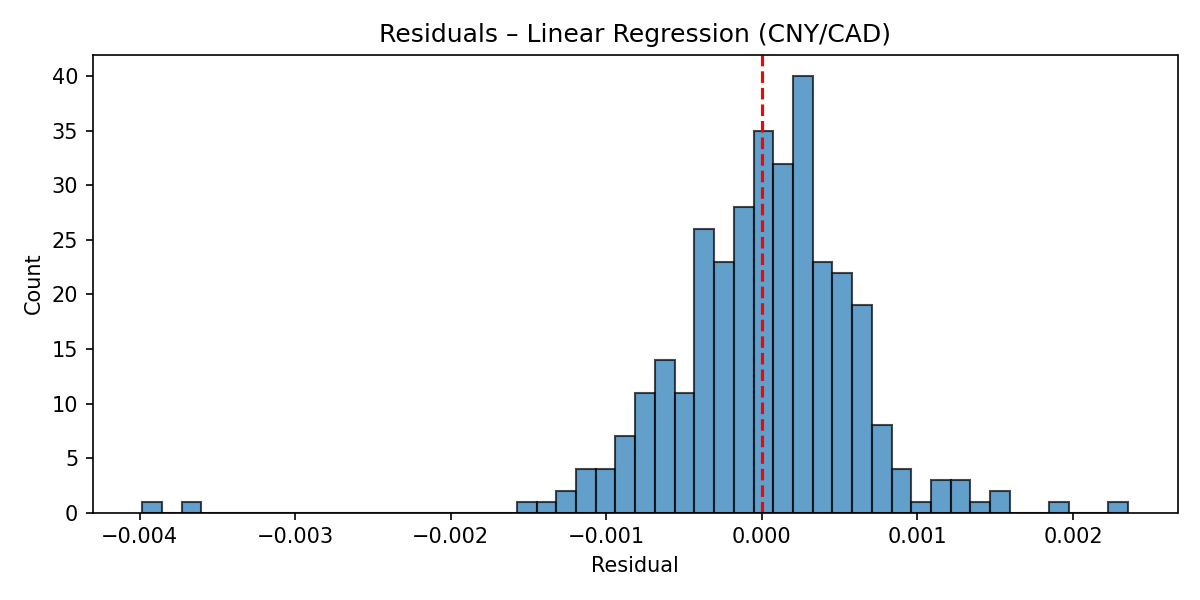
\includegraphics[width=\textwidth]{figures/CNY_Linear_Regression_residuals.png}
    \caption{LR -- CNY}
  \end{subfigure}\hfill
  \begin{subfigure}[b]{0.32\textwidth}
    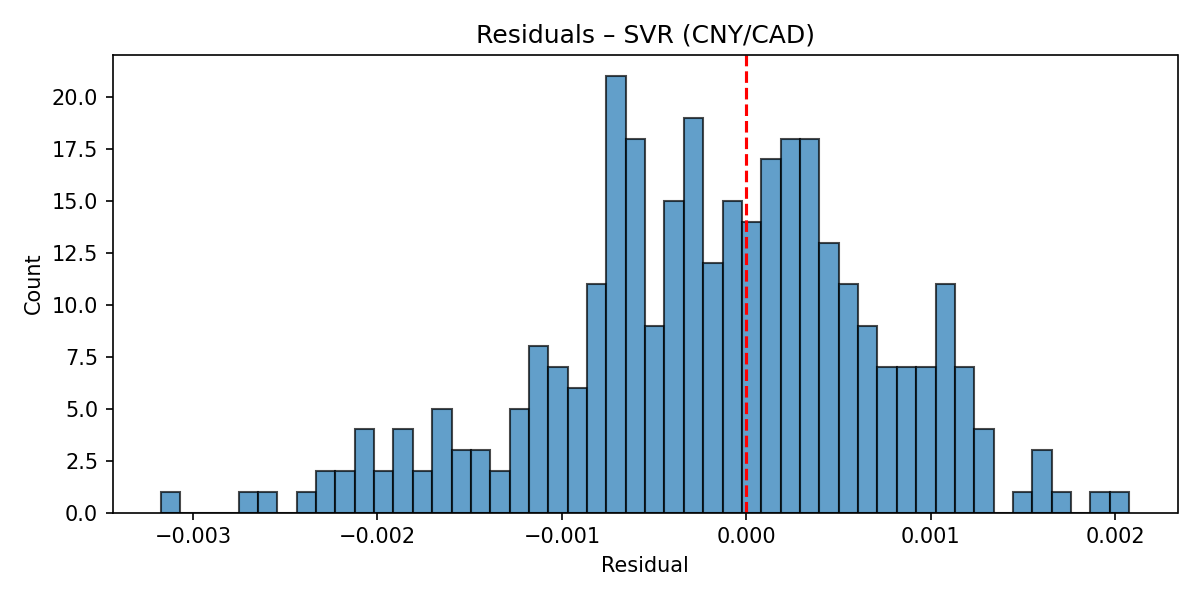
\includegraphics[width=\textwidth]{figures/CNY_SVR_residuals.png}
    \caption{SVR -- CNY}
  \end{subfigure}\hfill
  \begin{subfigure}[b]{0.32\textwidth}
    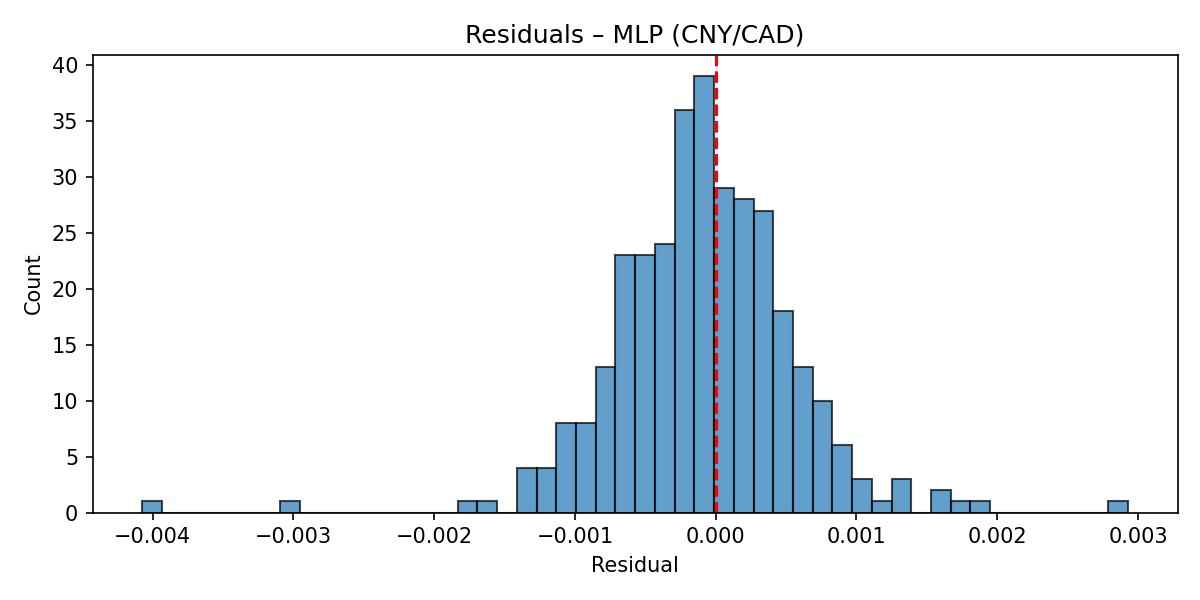
\includegraphics[width=\textwidth]{figures/CNY_MLP_residuals.png}
    \caption{MLP -- CNY}
  \end{subfigure}
  \caption{Residual histograms for all model--currency pair combinations. The red dashed line marks zero residual.}
  \label{fig:residuals}
\end{figure}

\subsection*{C. Source Code}

The code is organized as: \texttt{main.py} (entry point), \texttt{config.py} (hyperparameters), \texttt{src/data\_loader.py} (data download), \texttt{src/preprocessing.py} (features \& splitting), \texttt{src/models.py} (model definitions), \texttt{src/train.py} (training), \texttt{src/evaluate.py} (evaluation), \texttt{src/utils.py} (utilities). All figures are generated by running \texttt{python main.py}. Data from the Bank of Canada Valet API~[9] (public, no key required).


\newpage
\section*{AI Usage}

\section*{Contest for Information Sharing}
As part of this course, we may share selected project materials (e.g., reports, presentation slides, and presentation recordings) on the course webpage as learning resources for future students. Additionally, we may use anonymized project information for internal statistical analysis of course outcomes. Please indicate your preferences below. \textit{Your choices will not affect your grade in any way.}

\subsection*{Consent for Sharing Project Materials}
\textit{Please keep the item you wish and remove the other one.}

\begin{itemize}
	\item All group members consent to allow the project materials (report, slides, and presentation recording) to be shared on the course page for future students.
	%\item The group members do \textbf{not} consent to allow the project materials (report, slides, and presentation recording) to be shared on the course page for future students.
\end{itemize}

\subsection*{Consent for Use of Project Information in Statistical Analysis}
\textit{Please keep the item you wish and remove the other one.}
\begin{itemize}
	\item All group members consent to allow anonymized information about the project (e.g., topic, methods, outcomes, grades) to be used by the instructor for statistical analysis and course improvement.
	%\item The group members do \textbf{not} consent to allow anonymized information about the project (e.g., topic, methods, outcomes, grades) to be used by the instructor for statistical analysis and course improvement.
\end{itemize}

\subsection*{Optional Comments}
None.

\subsection*{Group Identification}

\begin{itemize}
	\item Group number: % TODO: fill in
	\item Names of group members: Member 1, Member 2, Member 3 % TODO: fill in real names
	\item Signature of group members: % TODO: sign
	\item Date: % TODO: fill in
\end{itemize}

\end{document}
